\section{Prototypes}\label{sec:sprint1-prototypes}
The first step in the project is to arrive at a common vision about the layout and functionality of the system.
To accomplish this, a series of wireframe prototypes were created.
A wireframe is a lo-fi prototyping technique where you create a grey box schematic that outlines the primary features of the user interface, unlike hi-fi prototypes which generally have a higher amount of detail and are used to test the interaction with the application.
The primary focus of these prototypes is not to be used for implementation, but rather for comparing opinions about how the flow in the system should be created.
Since the user interface is mostly focused on the mobile devices that the players will be wearing, it was decided that the host computer should simply have a text-based interface, as seen on \autoref{fig:prototype:hostlobby}.
\\\\
In terms of design considerations we considered the distinction between skeuomorphic and flat design.
Skeuomorphism is a term that describes interface objects that mimic their real-world counterparts in how they appear and are interacted with \cite{skeuomorphism}.
This design style is used to give context to users and ease them into using the design.
flat design, on the other hand, rejects 3D elements, which are likely to be used for skeuomorphic design, and focuses on rendering objects in a flat minimalist form.
The design we want to create for the game is a balance of these two styles.
While connecting to a game and finding a lobby, the design should be flat.
When the game is being played however, we adapt to a more skeuomorphic design to give the player an impression of what they are looking at and how to play.


\begin{figure}[H]
    \centering
    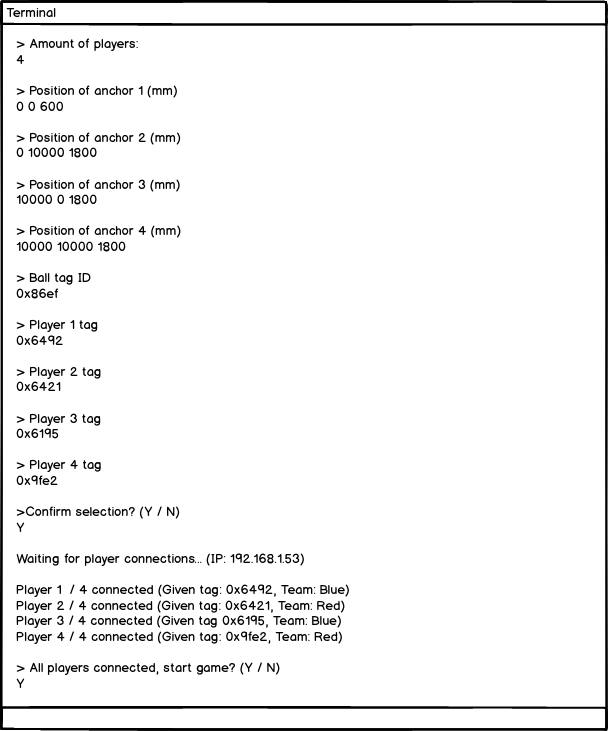
\includegraphics[width=0.6\linewidth]{prototypes/hostlobby.png}
    \caption{Prototype of hosting interface}
    \label{fig:prototype:hostlobby}
\end{figure}
\noindent
When a user starts the application, they will be greeted with an input field, where they will specify the IP address of the host machine, as seen on \autoref{fig:prototype:menu}. 

\begin{figure}[H]
    \centering
    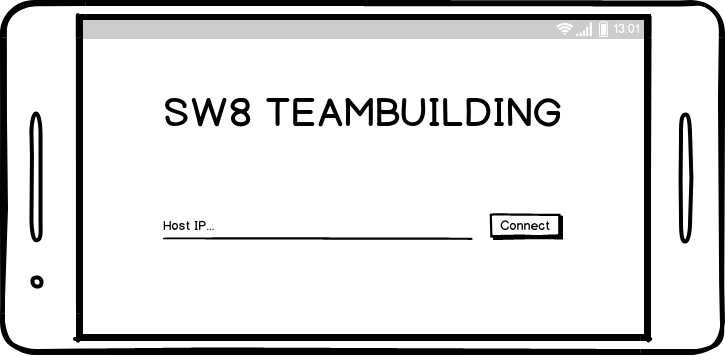
\includegraphics[width=0.6\linewidth]{prototypes/menu.png}
    \caption{Prototype of game menu}
    \label{fig:prototype:menu}
\end{figure}
\noindent
After inputting an IP and confirming, they will be redirected to a page where they can see how many users have connected to the host, as seen on \autoref{fig:prototype:menuconnected}. 

\begin{figure}[H]
    \centering
    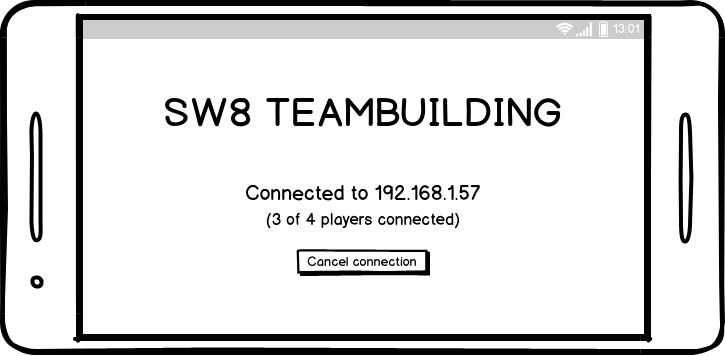
\includegraphics[width=0.6\linewidth]{prototypes/menuconnected.png}
    \caption{Prototype of screen where a user has connected to the host}
    \label{fig:prototype:menuconnected}
\end{figure}

\noindent
When all users have connected, the host can start the game, and they will now see the virtual game field, as seen on \autoref{fig:prototype:ingame}.
In this prototype, the players' icons are represented by small squares and the goals are represented by larger rectangles and have the same color as the players they belong to. \\
The current player's icon is highlighted by having a solid color, whereas the other players are just shown as outlines. 
The players are divided into two teams which are represented by the color of the player icons.
In the middle of the screen is the ball in a designated starting area to make the game fair for both teams.
This prototype iteration does not reflect the intended skeuomorphic design very well, since it is a lo-fi prototype.
However, care will be taken to for example make the field green during design, and having the ball represented by a regular ball design in the game.
\begin{figure}[H]
    \centering
    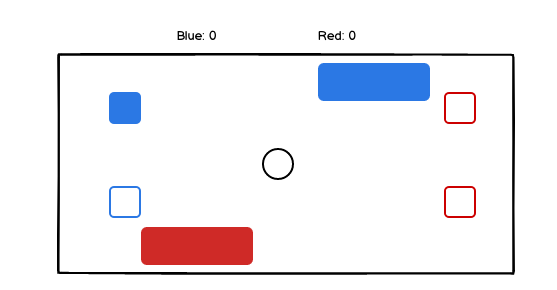
\includegraphics[width=0.6\linewidth]{prototypes/ingame.png}
    \caption{Prototype of in-game screen}
    \label{fig:prototype:ingame}
\end{figure}
